% Template for paper format at JPA
\documentclass[11pt,a4paper,xelatex,ja=standard]{bxjsarticle}
\geometry{left = 5.4cm, right = 5.4cm, top = 4.0cm, bottom = 3.5cm}
\renewcommand{\figurename}{Figure}
\renewcommand{\tablename}{Table}
\usepackage{lmodern}
\usepackage{amssymb,amsmath}
\usepackage{ifxetex,ifluatex}
\ifnum 0\ifxetex 1\fi\ifluatex 1\fi=0 % if pdftex
  \usepackage[T1]{fontenc}
  \usepackage[utf8]{inputenc}
  \usepackage{textcomp} % provide euro and other symbols
\else % if luatex or xetex
  \usepackage{unicode-math}
  \defaultfontfeatures{Scale=MatchLowercase}
  \defaultfontfeatures[\rmfamily]{Ligatures=TeX,Scale=1}
\fi
% Use upquote if available, for straight quotes in verbatim environments
\IfFileExists{upquote.sty}{\usepackage{upquote}}{}
\IfFileExists{microtype.sty}{% use microtype if available
  \usepackage[]{microtype}
  \UseMicrotypeSet[protrusion]{basicmath} % disable protrusion for tt fonts
}{}
\makeatletter
\@ifundefined{KOMAClassName}{% if non-KOMA class
  \IfFileExists{parskip.sty}{%
    \usepackage{parskip}
  }{% else
    \setlength{\parindent}{0pt}
    \setlength{\parskip}{6pt plus 2pt minus 1pt}}
}{% if KOMA class
  \KOMAoptions{parskip=half}}
\makeatother
\usepackage{xcolor}
\IfFileExists{xurl.sty}{\usepackage{xurl}}{} % add URL line breaks if available
\IfFileExists{bookmark.sty}{\usepackage{bookmark}}{\usepackage{hyperref}}
\hypersetup{
  pdftitle={RMarkdownで『心理学研究』の論文は書けるのか?},
  hidelinks,
  pdfcreator={LaTeX via pandoc}}
\urlstyle{same} % disable monospaced font for URLs
\usepackage{graphicx}
\makeatletter
\def\maxwidth{\ifdim\Gin@nat@width>\linewidth\linewidth\else\Gin@nat@width\fi}
\def\maxheight{\ifdim\Gin@nat@height>\textheight\textheight\else\Gin@nat@height\fi}
\makeatother
% Scale images if necessary, so that they will not overflow the page
% margins by default, and it is still possible to overwrite the defaults
% using explicit options in \includegraphics[width, height, ...]{}
\setkeys{Gin}{width=\maxwidth,height=\maxheight,keepaspectratio}
% Set default figure placement to htbp
\makeatletter
\def\fps@figure{htbp}
\makeatother
\setlength{\emergencystretch}{3em} % prevent overfull lines
\providecommand{\tightlist}{%
  \setlength{\itemsep}{0pt}\setlength{\parskip}{0pt}}
\setcounter{secnumdepth}{-\maxdimen} % remove section numbering
\usepackage{booktabs}
\usepackage{longtable}
\usepackage{array}
\usepackage{multirow}
\usepackage{wrapfig}
\usepackage{float}
\usepackage{colortbl}
\usepackage{pdflscape}
\usepackage{tabu}
\usepackage{threeparttable}
\usepackage{threeparttablex}
\usepackage[normalem]{ulem}
\usepackage{makecell}
\title{RMarkdownで『心理学研究』の論文は書けるのか?}
\usepackage{etoolbox}
\makeatletter
\providecommand{\subtitle}[1]{% add subtitle to \maketitle
  \apptocmd{\@title}{\par {\large #1 \par}}{}{}
}
\makeatother
\subtitle{Can we write a paper of the Japanses Journal of psychology with
RMarkdown?}
\author{}
\date{}
\usepackage{marginnote}
\usepackage{titlesec}
\titleformat{\section}[hang]{\large\filcenter\bfseries}{\thesection}{1zw}{}

\begin{document}
\pagestyle{empty}
\maketitle
\pagestyle{plain}
\setcounter{page}{1}

\hypertarget{abstract}{%
\section{Abstract}\label{abstract}}

Can we write a paper of the Japanses Journal of psychology with
RMarkdown? To solve this mystery we headed deep into the Amazon. At the
end of our long journey we found some great documents about RMarkdown
and finally said, ``Yes, we can''. \ldots{} Well, we'll write a abstract
like this.

\textbf{Key words}: RMarkdown, Reproducibility, The Japanese Journal of
Psychology

\clearpage

 はじめに,ここから文章を書き始めます。以降が論文の本文になります。どんどん書いていきましょう!

\hypertarget{ux5fc3ux7406ux5b66ux306bux304aux3051ux308bux518dux73feux53efux80fdux6027}{%
\subsection{心理学における再現可能性}\label{ux5fc3ux7406ux5b66ux306bux304aux3051ux308bux518dux73feux53efux80fdux6027}}

 心理学の再現可能性はとってもまずい状況なのですが,それはちょっとおいておいて,文献の引用の仕方を説明します。まず,Kunisato
et al. (2012)
のように,すると,bibファイル内のKunisatoの2012年の論文が引用されます。そして,次のように,{[}{]}でくくると文末の引用スタイルになります(国里愛彦・片平健太郎・沖村宰・山下祐一,
2019)。また,文末に複数引用する場合は,こういう感じにします(Machino et
al., 2014; 国里愛彦・片平健太郎・沖村宰・山下祐一,
2019)。以下に詳しく書いているのでご確認ください。  

 続いて,論文では脚注をつけることがあります。その場合は,このように上付き文字をつけます\({}^1\)。心理学研究では,引用文献の後ろに脚注をつけることになっているので,ここでつけた上付き文字に対応したものを書き込んでおきます。まあ,こんなに短い距離で2つも脚注とかつけないわけですが,練習のために,もう一つつけます\({}^2\)。

\clearpage

12345678901234567890123456789012345678901234567890123456789012345678901234567890123456789012345678901234567890123456789012345678901234567890123456789012345678901234567890123456789012345678901234567890123456789012345678901234567890123456789012345678901234567890123456789012345678901234567890123456789012345678901234567890123456789012345678901234567890123456789012345678901234567890123456789012345678901234567890123456789012345678901234567890123456789012345678901234567890123456789012345678901234567890123456789012345678901234567890123456789012345678901234567890123456789012345678901234567890123456789012345678901234567890123456789012345678901234567890123456789012345678901234567890123456789012345678901234567890123456789012345678901234567890123456789012345678901234567890123456789012345678901234567890

\hypertarget{rmarkdownux3068ux306f}{%
\subsection{RMarkdownとは}\label{rmarkdownux3068ux306f}}

 RMarkdownは,RとMarkdownが合体したもので,Markdownは簡単に言うとLaTeXよりも簡単にかけるやつです。RMarkdownで書いてPDF出力する際には,LaTeXを経由します。でも,数式を書いたり,ちょっと特殊なことをしない限りは,ユーザーはLaTeXを意識せずにきれいな論文を書くことができます。

\hypertarget{ux672cux7814ux7a76ux306eux76eeux7684}{%
\subsection{本研究の目的}\label{ux672cux7814ux7a76ux306eux76eeux7684}}

 
 RMarkdownでちゃんと『心理学研究』に投稿できる原稿PDFファイルが作れるか検証した。

\hypertarget{ux65b9-ux6cd5}{%
\section{方 法}\label{ux65b9-ux6cd5}}

\hypertarget{ux53c2ux52a0ux8005}{%
\subsection{参加者}\label{ux53c2ux52a0ux8005}}

 神奈川県内の私立大学生2800名(男性919名,女性1881名)が調査に参加した。参加者の平均年齢
(標準偏差) は,28.78歳(11.13)であった。

\hypertarget{ux4f7fux7528ux5909ux6570}{%
\subsection{使用変数}\label{ux4f7fux7528ux5909ux6570}}

\textbf{心理学再現性確認尺度} 心理学研究の場合,見出しじゃなくて太字にしたい時というがあると思います。左の心理学再現性確認尺度のように,アスタリスク2つではさむとそれができます。

 論文では,図を挿入したりするのですが,その図の挿入箇所の指示を余白ですることが多いです。例えば,Figure
1をこの辺に挿入しようかなというときは,\marginpar{\fbox{Figure 1}}こういう感じでLatexのmarginparパッケージとfboxを活用して,Figure
1を線で囲ったものを作ります。

\hypertarget{ux8abfux67fbux624bux7d9aux304d}{%
\subsection{調査手続き}\label{ux8abfux67fbux624bux7d9aux304d}}

 見出しは適当につけているので,調査手続きにしたり,実験手続きにしたり変更ください。

\hypertarget{ux7d71ux8a08ux89e3ux6790}{%
\subsection{統計解析}\label{ux7d71ux8a08ux89e3ux6790}}

 統計解析について必要に応じて記載ください。Rパッケージなどのオープンソースソフトウェアは無料ですが,だからこそ,その公開した方の科学への貢献に感謝し,適切に引用しましょう。

\hypertarget{ux7d50-ux679c}{%
\section{結 果}\label{ux7d50-ux679c}}

 論文では,表を挿入したりするのですが,その表の挿入箇所の指示を余白ですることが多いです。例えば,Table1をこの辺に挿入しようかなというときは,\marginpar{\fbox{Table1}}こういう感じでLatexのmarginparパッケージとfboxを活用して,Table1を線で囲ったものを作ります。

\hypertarget{ux5916ux5411ux6027ux3068ux795eux7d4cux75c7ux50beux5411ux306eux95a2ux9023}{%
\subsection{外向性と神経症傾向の関連}\label{ux5916ux5411ux6027ux3068ux795eux7d4cux75c7ux50beux5411ux306eux95a2ux9023}}

 練習で,psychパッケージのbfiを用いて,外向性と神経症傾向を算出してみましょう。外向性と神経症傾向のPearsonの積率相違関係数は,0.038であり(\emph{t}(2615)
= 1.968, \emph{p} = 0.049,その95\%信頼区間は,0.000から0.077です。
 散布図は,Figure 2に示す\marginpar{\fbox{Figure 2}}。

\hypertarget{ux8003-ux5bdf}{%
\section{考 察}\label{ux8003-ux5bdf}}

 本研究では,RMarkdownで『心理学研究論文』がかけるのかを検証した。それ用のテンプレートも用意したので,あとは解析と内容を書くだけで結構いい感じのものができる。ただし,引用文献については,まだ完全とはいえず,共にこのテンプレートを磨く有志を心待ちしている。

\clearpage

\hypertarget{ux5f15ux7528ux6587ux732e}{%
\section{引用文献}\label{ux5f15ux7528ux6587ux732e}}

\hypertarget{refs}{}
\leavevmode\hypertarget{ref-Kunisato2012}{}%
Kunisato, Y., Okamoto, Y., Ueda, K., Onoda, K., Okada, G., Yoshimura,
S., \ldots{} Yamawaki, S. (2012). Effects of depression on reward-based
decision making and variability of action in probabilistic learning.
\emph{Journal of Behavior Therapy and Experimental Psychiatry},
\emph{43}(4), 1088--1094.

\leavevmode\hypertarget{ref-Machino2014}{}%
Machino, A., Kunisato, Y., Matsumoto, T., Yoshimura, S., Ueda, K.,
Yamawaki, Y., \ldots{} Yamawaki, S. (2014). Possible involvement of
rumination in gray matter abnormalities in persistent symptoms of major
depression: An exploratory magnetic resonance imaging voxel-based
morphometry study. \emph{Journal of Affective Disorders}, \emph{168},
229--235.

\leavevmode\hypertarget{ref-kunisato2019}{}%
国里愛彦・片平健太郎・沖村宰・山下祐一. (2019).
うつに対する計算論的アプローチ:―強化学習モデルの観点から―.
\emph{心理学評論}, \emph{62}(1), 88--103.
\url{https://doi.org/10.24602/sjpr.62.1_88}

\clearpage

\hypertarget{ux811aux6ce8}{%
\section{脚注}\label{ux811aux6ce8}}

\({}^1\)脚注の例1です。論文の補足をどうぞ。

\({}^2\)脚注の例2です。

\clearpage 
\newgeometry{left = 3cm, right = 3cm, top = 3cm, bottom = 3cm}

\hypertarget{ux8868}{%
\section{表}\label{ux8868}}

\begin{table}[!h]

\caption{\label{tab:unnamed-chunk-4}Descriptive Statistics of bfi}
\centering
\begin{tabular}[t]{lrrrrrrrr}
\toprule
  & n & Mean & SD & Median & Min & Max & Skewness & kurtosis\\
\midrule
\cellcolor{gray!6}{Extraversion} & \cellcolor{gray!6}{2713} & \cellcolor{gray!6}{18.96} & \cellcolor{gray!6}{2.71} & \cellcolor{gray!6}{19} & \cellcolor{gray!6}{5} & \cellcolor{gray!6}{29} & \cellcolor{gray!6}{0.01} & \cellcolor{gray!6}{1.08}\\
Neuroticism & 2694 & 15.82 & 5.97 & 15 & 5 & 30 & 0.22 & -0.66\\
\cellcolor{gray!6}{Conscientiousness} & \cellcolor{gray!6}{2707} & \cellcolor{gray!6}{19.04} & \cellcolor{gray!6}{2.77} & \cellcolor{gray!6}{19} & \cellcolor{gray!6}{5} & \cellcolor{gray!6}{30} & \cellcolor{gray!6}{-0.17} & \cellcolor{gray!6}{0.81}\\
Agreeableness & 2709 & 21.04 & 3.68 & 22 & 5 & 30 & -0.66 & 0.68\\
\cellcolor{gray!6}{Openness} & \cellcolor{gray!6}{2726} & \cellcolor{gray!6}{19.34} & \cellcolor{gray!6}{2.74} & \cellcolor{gray!6}{19} & \cellcolor{gray!6}{5} & \cellcolor{gray!6}{29} & \cellcolor{gray!6}{-0.02} & \cellcolor{gray!6}{1.09}\\
\bottomrule
\multicolumn{9}{l}{\textsuperscript{a} Note. SD=standard deviation}\\
\end{tabular}
\end{table}

\clearpage

\hypertarget{ux56f3}{%
\section{図}\label{ux56f3}}

\begin{figure}
\centering
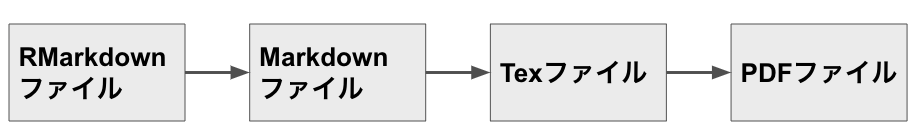
\includegraphics{fig1.png}
\caption{How R Markdown works}
\end{figure}

\clearpage

\begin{figure}
\centering
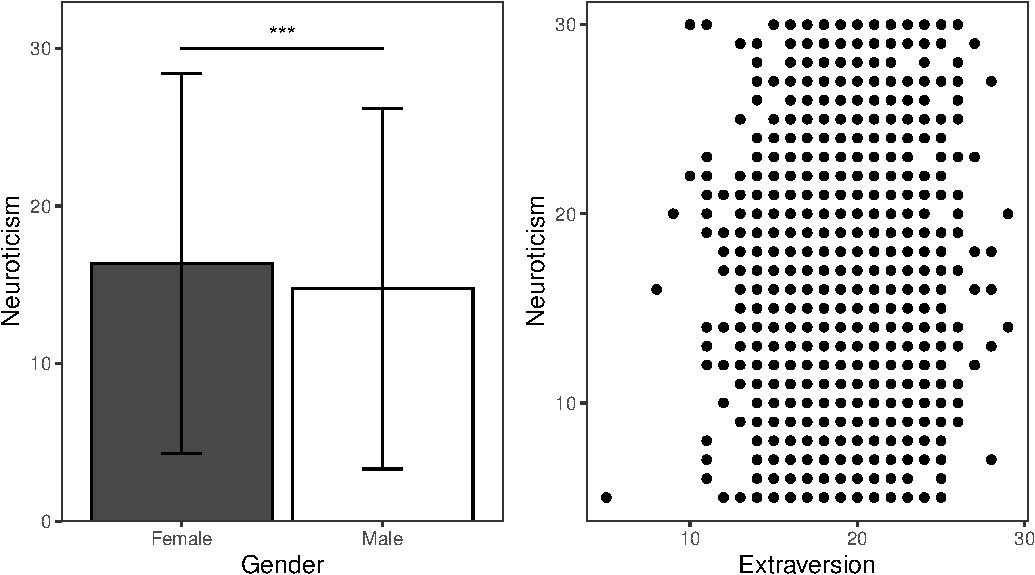
\includegraphics{test_files/figure-latex/figs-1.pdf}
\caption{\label{fig:figs}Examples of bar plot and scatter plot}
\end{figure}

\clearpage

\hypertarget{ux4ed8ux9332}{%
\section{付録}\label{ux4ed8ux9332}}

新たに質問紙を作成したら,どこかで使った質問票を公開してほしい・・・

\end{document}
